\providecommand{\relativeRoot}{../..}
\documentclass[\relativeRoot/main.tex]{subfiles}
\graphicspath{{\subfix{./figures/}}}


\begin{document}

\section{Motivation}
\label{sec:lyprox:motivation}

Publishing and sharing the data of \cref{chap:dataset_usz} with the scientific community is a valuable contribution, since it allows other researchers to test a range of hypotheses. For example, one might be interested in how the involvement of upstream \glspl{lnl} influences the risk of nodal metastases in a given level. Something we have given an answer to in \cref{table:dataset_usz:upstream}. But also theories we did not think of at the time of writing our publications \cite{ludwig_detailed_2021,ludwig_dataset_2021} may be tested by someone who searches the literature for support in favor or against a particular hypothesis.

However, in such a case there are still some hurdles to discovering and taking advantage of freely available data: The researcher -- who we assume to have already conceived their hypothesis -- needs to understand what is reported in the dataset, what format it is provided in and how to implement a test using the found information. Our data is provided as a \gls{csv} table, meaning it can be opened in a spreadsheet program like Microsoft Excel. This would allow the user to create e.g. pivot tables and derived variables from observed ones, after they have made themselves familiar with the description and meaning of all the provided columns.

Taking these steps is not particularly difficult, and a determined scientist may be able to accomplish that in a matter of hours. However, if a researcher came up with a quick idea, not yet fully developed into a hypothesis, the outlined procedure could -- in their eyes -- very well not be worth the potential insight. Consequently, an interesting idea and a valuable cohort of patients might be left unexplored. Even more so with someone who did not even come up with a research question our data may be able to answer.

Figures and tables, like \cref{fig:dataset_usz:statistics} and \cref{table:dataset_usz:prevalences} that allow a reader of our work to quickly and visually understand our data address these issues to some extent. They create an understanding of what is reported in the data and answer common questions about it. But it is not feasible to provide plots and tables on all aspects of a dataset within a publication.

\subsection*{Prototype}
\label{subsec:lyprox:motivation:prototype}

This is precisely why we thought of creating a dashboard, allowing a user to create the visualizations and numbers themselves according to their interest w.r.t. the underlying data. The first implementation that provided such a dashboard was a Python-based \gls{gui} developed by Bertrand Pouymayou for the use on local hardware (e.g. a laptop). It could display the prevalence of involvement for all \glspl{lnl} while the patients could be stratified by a number of reported variables that were recorded (e.g. smoking status). Moreover, one could explore how frequently certain levels were involved together or on their own, e.g. without metastases in upstream \glspl{lnl}. A screenshot of this first prototype is shown in \cref{fig:lyprox:pouymayou_gui}.

\begin{figure}
    \centering
    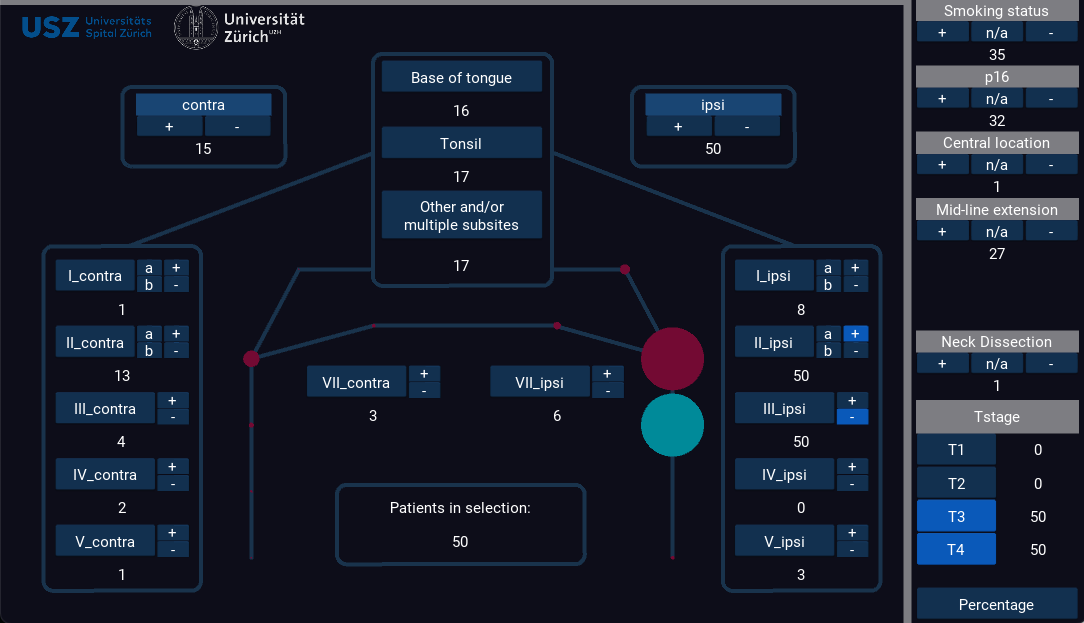
\includegraphics[width=1.0\textwidth]{figures/pouymayou_gui.png}
    \caption[
        Prototype of a GUI to explore patterns of lymphatic progression
    ]{
        Python-based \gls{gui} as developed by Bertrand Pouymayou to interactively explore our dataset containing patterns of lymphatic progression. The sidebar on the right allows stratification w.r.t. patient and tumor information, e.g. smoking status, lateralization of the primary tumor or T-stage. In the center, patients can be selected based in primary tumor subsites. The boxes named e.g. \texttt{III\_ipsi} allowed to (de)select patients with metastases in the respective \gls{lnl}.
    }
    \label{fig:lyprox:pouymayou_gui}
\end{figure}

\end{document}
